\chapter{Monitor}

\section{Introduzione}

\paragraph{Problemi dei semafori:}

\begin{itemize}
	\item Basilari, poco strutturati e poco sicuri.
	\item La correttezza è onere del programmatore.
	\item Il linguaggio di programmazione tipicamente non fornisce un modo per
	      strutturare l’uso dei semafori (eccetto la mutua esclusione), perché
	      l’uso può richiede un’interazione elaborata tra frammenti di codice di
	      processi diversi.
\end{itemize}

\dfn{Monitor}{
	Il monitor è un costrutto strutturato per linguaggi di alto livello. Si tratta di un costrutto sintattico che associa un insieme di operazioni a una struttura dati condivisa da più processi.
}

\nt{Sulla struttura dati del monitor si agisce solamente attraverso operazioni definite \fancyglitter{mutuamente esclusive} (un solo proceso per volta è attivo nel monitor).}

\subsection{Definire un Monitor}

\begin{center}
	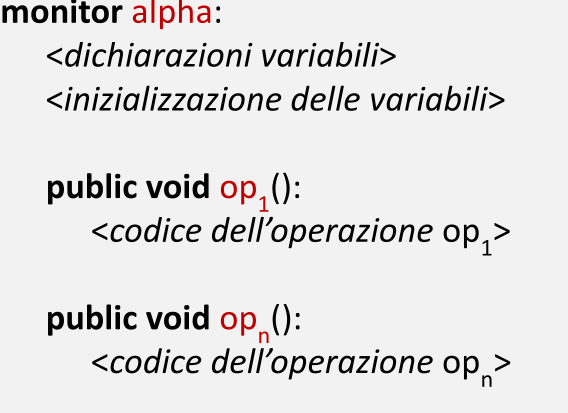
\includegraphics[scale=0.4]{04-Monitor/m.png}
\end{center}

\paragraph{Definizione di monitor:}

\begin{itemize}
	\item Le operazioni public sono le sole operazioni che possono
	      essere utilizzate dai processi per accedere alla struttura dati
	      condivisa.
	\item Le variabili condivise mantengono il loro valore tra
	      successive esecuzioni delle operazioni del monitor (\fancyglitter{variabili
		      permanenti}).
	\item Le variabili condivise sono \fancyglitter{accessibili solo dai metodi del
		      monitor} (sono private).
	\item Le operazioni non dichiarate public \fancyglitter{non sono accessibili
		      dall’esterno}. Sono usabili solo dalle funzioni public.
\end{itemize}

\paragraph{Dichiarazione di un monitor:}

\begin{itemize}
	\item La definizione di un monitor (monitor alpha:\dots) definisce un \fancyglitter{tipo} (alpha).
	\item Per creare un'\fancyglitter{istanza} del monitor occorre definire una variabile con quel tipo (alpha x).
	\item Per chiamare un'operazione \fancyglitter{$op_i$} si utilizza la dot notation ($x.op_i$()).
\end{itemize}

\begin{center}
	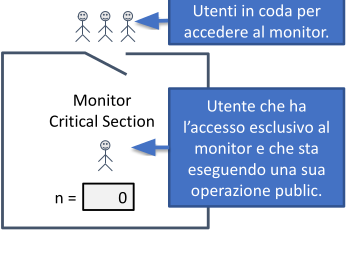
\includegraphics[scale=0.4]{04-Monitor/mcs.png}
\end{center}

\clm{}{}{
	\begin{itemize}
		\item Il monitor è un'\fancyglitter{entità statica}: un insieme di procedure che possono essere richiamate dai singoli processi  che condividono dei dati permanenti.
		\item \fancyglitter{Lock}: meccanismo che garantisce che un solo processo per volta sia all'interno del monitor in un certo istante.
	\end{itemize}
}

\subsection{Variabili di Condizione}

\dfn{Variabile di Condizione}{
	Una variabile di condizione  permette la sospensione di un processo all'interno del monitor nel caso in cui si debba verificare una condizione.
}

\clm{}{}{
	\begin{itemize}
		\item La dichiarazione di una variabile x di tipo \fancyglitter{condition} ha la forma: condition x.
		\item Ogni variabile di tipo condition rappresenta una \fancyglitter{coda FIFO} nella quale i processi si possono sospendere.
		\item Le procedure del monitor agiscono su tali variabili con due operazioni:
		      \begin{itemize}
			      \item wait(x). Sospende il processo e lo mette nella coda x.
			      \item signal(x). Risveglia il primo processo in attesa nella coda x se esiste.
		      \end{itemize}
	\end{itemize}
}

\paragraph{Wait(x):}

\begin{enumerate}
	\item Inserisce il processo q al fondo della coda.
	\item Pone lo stato di q a "blocked".
	\item Rilascia il controllo del monitor.
\end{enumerate}

\paragraph{Signal(x) (se la coda non è vuota):}

\begin{enumerate}
	\item Preleva il primo processo p presente in coda.
	\item Pone lo stato di p a "ready".
	\item Continua nel monitor.
\end{enumerate}

\begin{center}
	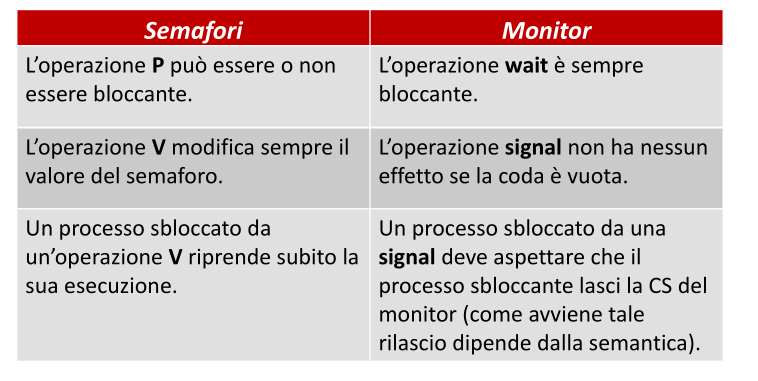
\includegraphics[scale=0.4]{04-Monitor/svm.png}
\end{center}

\paragraph{Tipi di semantiche per l'operazione signal:}

\begin{itemize}
	\item signal\_and\_continue: il processo svegliante continua l'esecuzione, mentre il processo svegliato si pone in attesa di entrare nel monitor.
	\item signal\_and\_wait: il processo svegliato riprende immediatamente
	      l’esecuzione, mentre il processo svegliante si pone in attesa di rientrare
	      nel monitor.
	\item signal\_and\_urgent\_wait: il processo svegliato riprende l’esecuzione,
	      mentre il processo svegliante si pone in attesa di rientrare nel monitor
	      in una coda ad alta priorità (\fancyglitter{urgent queue}). Questa politica viene anche
	      detta immediate resumption requirement (IRR) ed è l’implementazione
	      classica.
\end{itemize}

\paragraph{Ulteriori operazioni:}

\begin{itemize}
	\item empty(x): restituisce true se la coda e vuota, false altrimenti.
	\item signal\_all(cond): risveglia tutti i processi sospesi sulla variabile cond (si può usare solo con semantica signal\_and\_continue).
\end{itemize}

\qs{}{I monitor e i semafori hanno la stessa capacità di sincronizzazione? Ogni problema di sincronizzazione
	che si può risolvere con i semafori si può risolvere anche con il
	monitor e viceversa?}

\paragraph{Risposta:} sì, la dimostrazione si fa costruendo un semaforo con un monitor e costruendo un monitor con un semaforo.

\section{Invarianti di Monitor}

\dfn{Invariante di Monitor}{
	Un Invariante di monitor IM è una proposizione che risulta soddisfatta immediatamente prima e subito dopo ogni operazione del monitor.
}

\nt{L'invariante non è necessariamente soddisfatto durante l'operazione del monitor.}

\paragraph{Per dimostrare che una proposizione IM è un invariante di monitor è sufficiente verificare che:}

\begin{itemize}
	\item \fancyglitter{Passo base:} la proposizione IM è vera al momento dell'inizializzazione del monitor.
	\item \fancyglitter{Passo induttivo:} supposta IM vera all’inizio della chiamata di un’operazione di monitor, si prova che IM è vera anche all’uscita dal monitor alla fine dell’esecuzione della stessa operazione.
\end{itemize}

\paragraph{Per esempio, per provare la correttezza nel problema dei lettori/scrittori:}

\begin{itemize}
	\item R: numero dei processi lettori che stanno leggendo, cioè
	      hanno completato l’operazione di inizio\_lettura e
	      non hanno ancora invocato la fine\_lettura.
	\item W: numero dei processi scrittori che stanno scrivendo, cioè
	      hanno completato l’operazione di inizio\_scrittura e
	      non hanno ancora invocato la fine\_scrittura.
	\item Invariante: $R > 0 \rightarrow W = 0 \land (W \leq 1) \land (W = 1 \rightarrow R = 0)$:
	      \begin{itemize}
		      \item $R > 0 \rightarrow W = 0$: se ci sono lettori attivi non possono esserci scrittori attivi.
		      \item $(W \leq 1)$: al massimo uno scrittore può essere attivo.
		      \item $(W = 1 \rightarrow R = 0)$: se c'è uno scrittore attivo non possono esserci lettori attivi.
	      \end{itemize}
\end{itemize}



